\documentclass[12pt]{article}
\usepackage{latexsym}
\usepackage{amssymb,amsmath}
\usepackage[pdftex]{graphicx}
\usepackage{epstopdf}
\usepackage{MnSymbol,wasysym}


\topmargin = 0.1in \textwidth=5.7in \textheight=8.6in

\oddsidemargin = 0.2in \evensidemargin = 0.2in


\begin{document}

\begin{center}
COMPUTER SCIENCE 20, SPRING 2014 \\
Week 8 Homework Problems\\
Undirected Graphs and Connectivity \\
Author: Tawheed Abdul-Raheem
\end{center}

\smallskip

\begin{enumerate}
\item Consider a group of 5 people. Within the group Amy knows 3 other people, Bob knows 4, Cal knows 4, Dan knows at least one, and Eva knows at least one.

How many people in the group does each of Dan and Eva know? List all the possible values, and prove that there are no others.

\begin{displaymath}
\begin{array}{|c|c|c|c|c|}
    Amy & Bob &  Cal & Dan & Eva \\
\hline
Bob & Cal  &  Bob &  Bob & Bob   \\
Cal  & Dan  &  Dan &  Cal & Cal   \\
Dan / Eva  & Eva  &  Eva &  Amy & Amy   \\
 & Amy  &  Amy &  Eva &  Dan \\
\end{array}
\end{displaymath}

Because Amy knows three people it could be the case that she might know either Dan or Eva, doing so will increase the number of people that Dan and Eva know. The possible number of people that each of them may know is 4. 
\item Show that graphs 1 and 2 are isomorphic, and show that graphs 3 and 4 are not isomorphic.

\begin{center}
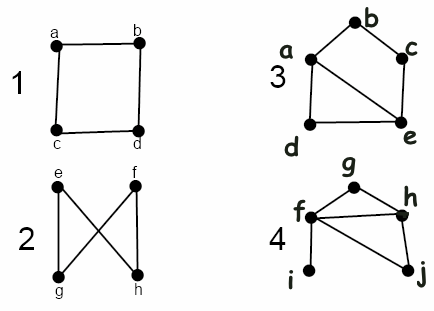
\includegraphics[scale=0.8]{sample.png}
\end{center}

\textbf{1} and \textbf{2} are isomorphic because they have equal amount of nodes which  is $4$ and they all so have the same number of degree vertex. Another important property is that the mapping from $G(1)$ to $G(2)$ preserves the number of incident edges. Below is the degree of vertex for $1$ and $2$. For graph 1, degree of vertex $a=2, b=2, c=2, d=2$ and graph 2, degree of vertex $e=2, f=2, g=2, h=2$ \\

\textbf{3} and \textbf{4} are not isomorphic, although they have the same number of nodes the number of vertex of each node in both graph are different. These are the degree vertex for graph \textbf{3} and \textbf{4}, $G(3) $ has $b=2, a=3, d=2, e=3, c=2$ and $G(4)$ has $g=2, f=4, h=3, j=2, i=1$. Finally the mapping between $G(3)$ and $G(4)$ does not preserve the edges when they are mapped to each other.

Isomorphism graphs can be mapped one-to-one and also it preserves the degree of the edges.
\item A tree is an undirected graph in which any two vertices are connected by exactly one path (i.e.~a graph with no cycles).  
\begin{enumerate}
\item Prove for a tree $G=(V,E)$ by induction on $|V|$ that $|E|=|V|-1$. \\
    Let $P(n)$ be the proposition that every graph $G$ with $n$ number of vertex has  $|E|=|V|-1$ \\
    \textbf{\textit{Base case: }} There exists a single $V$ in our graph, by definition we know that a one-node tree has no edges \\
    \textbf{\textit{Inductive Step: }} We assume that exists a graph with $n+1$ vertices, and prove that the graph has $(n+1)-1$ edges. If we remove one node from the tree, we also have to remove one edge because an edge connects two vertices/nodes. By induction we know that a graph of $1$ node does not have any edges. Now if we put that node back to our tree, our $E$ will be restored.
    
\item Prove that the edge and vertex connectivity of any tree are both $1$. Hint: Prove first by induction that every tree contains some vertex of degree $1$.\\
    \textbf{\textit{Base case: }} A two node tree (has no cycles) has an edge and vertex connectivity of 1. For an edge to be valid it must connect two nodes.
    \textbf{\textit{Inductive Step: }} We assume that our base case is true inorder to prove for $n+1$ vertices in a tree. If we add a new node to our tree, the vertex connectivity of that tree with the tree that already exists must has a maximum edge of $1$. If on the other hand we adding a new vertex to the tree allows have to have an edge of more than $1$ it will mean that there exists a cycle which no longer becomes a valid tree.

\end{enumerate}
\item A \emph{spanning tree} of a graph $G=(V,E)$ is a tree on the set of all vertices of $G$ whose edges are in $E$. In other words, it is a tree that connects all the vertices of $G$ using only edges in $G$.
\begin{enumerate}
\item Prove or disprove: For a given a graph $G$, any two spanning trees of $G$ are isomorphic. \\
    For any given graph $G$, any two spanning trees of that graph is isomorphic. Lets take the fist spanning tree of our graph $G$, we know that inorder for it to be a valid spanning tree it must not have a cycle. Thus for a graph $G$ with $n$ vertices, the valid spanning tree mmust be $n-1$. Now if we take another spanning tree from that same graph $G$. It must be the case that it is isomorphic with the first tree because it would have the same nodes and the same number of degree of vertices. If the second graph however has a degree that does not match the first one, then it must be the case that the second tree has a cycle.
\item How many spanning trees are there for the complete graphs $K_2$, $K_3$, $K_4$, and $K_5$? For $K_5$, there are quite a few, so don't write them out. Instead, just describe how you counted them. Sorting by isomorphism classes may be useful. For example, there are $60$ spanning trees of $K_5$ that are isomorphic to the path $P_5$. \\
    $K_2 = 1, K_3 = 3, K_4 = 16, K_5 = 125$
\item Conjecture (but do not prove) a general formula for the number of spanning trees of $K_n$. Your answer will be judged as correct if it matches the values you obtained in part (b).\\
    The general formular for finding the number of spanning tree in graph is $K_n = n^{n-2}$
\end{enumerate}
\end{enumerate}


\end{document}
